\documentclass[compress,11pt]{beamer}
%\includeonly{pendel}
\usetheme{Ilmenau}
%\usetheme{fau-4-3}
%\usecolortheme{beaver}
\beamertemplatenavigationsymbolsempty
\usepackage[ngerman]{babel}
\usepackage{marvosym}
\usepackage{multimedia}
\usepackage[utf8]{inputenc}
\usepackage{amsmath}
\usepackage{amsfonts}
\usepackage{amssymb}
\usepackage{graphicx}
\usepackage{esvect}
%\author{}
\title{EP Gruppe 8}
%\setbeamercovered{transparent}
%\setbeamertemplate{navigation symbols}{}
%\logo{}
%\institute{}
%\date{}
%\subject{}
\usepackage{verbatim}
\begin{document}

\section{Aufgabe 1}
\begin{frame}
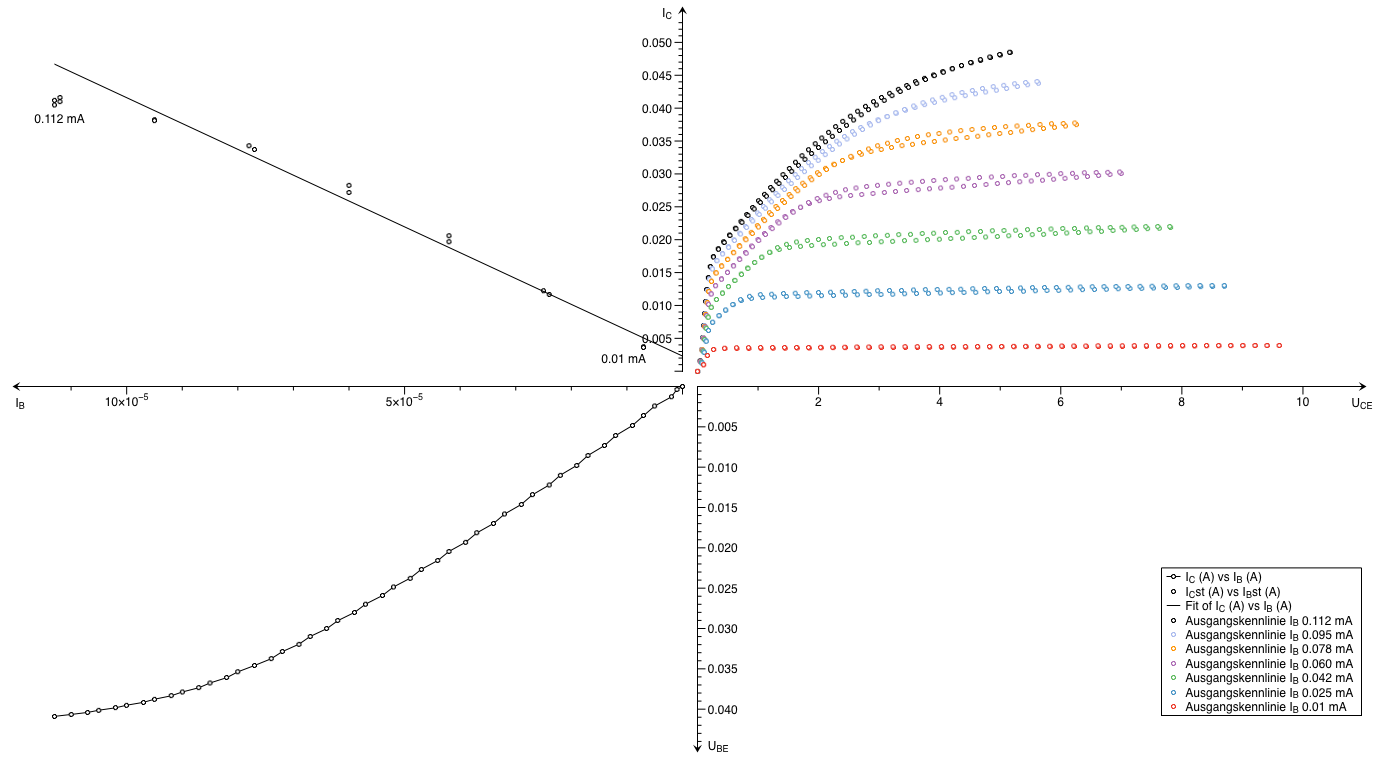
\includegraphics[width=1.1\textwidth]{kennlinienfeld.png}
\end{frame}
\begin{frame}
\begin{block}{Warum unterscheiden sich Hoch- und Rückregelung der Ausgangskennlinien }
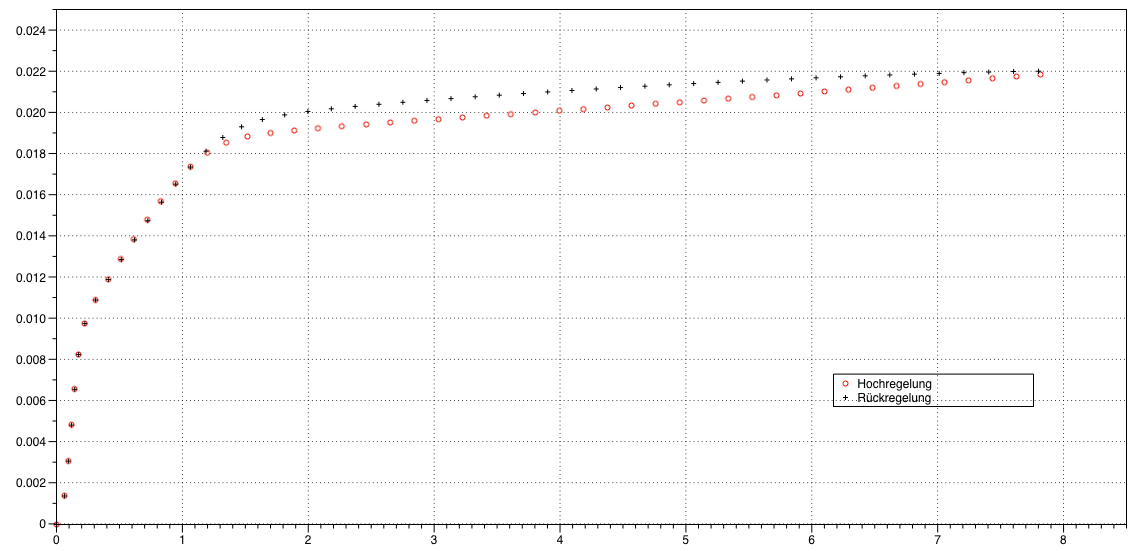
\includegraphics[width=\textwidth]{hinruck.png}
\end{block}
\end{frame}
\begin{frame}
\begin{block}{Warum unterscheiden sich Hoch- und Rückregelung der Ausgangskennlinien }
Beim Hochregeln wird der Transistor aufgewärmt beim Rückregeln ist der Transistor damit wärmer und es kann mehr Strom fliesen
\end{block}
\end{frame}

\section{Aufgabe 2}
\begin{frame}
%\includegraphics schaltung
%\end{frame}
%\begin{frame}
\subsection{Erste Version der Schaltung}
\begin{itemize}
\item Transistor hier als Schalter, da Strom nur fließt, wenn $U_{CE} \neq 0$
\item Sobald der Schalter in der ersten Schaltung geschlossen ist, liegt an Collector und Emitter eine Spannung an und der Transistor lässt durch $\Rightarrow$ iode leuchtet
\end{itemize}
\subsection{Zweite Version der Schaltung}
\begin{itemize}
\item Jetzt liegt konstante Spannung an Collektor und Emitter $\Rightarrow$ Transistor sperrt nicht und Diode leuchtet
\item Schaltung
\end{itemize}
\end{frame}
\subsection{Darlington-Schaltung}
\begin{frame}
	\begin{columns}
	\column{.48\textwidth}
	%\centering
	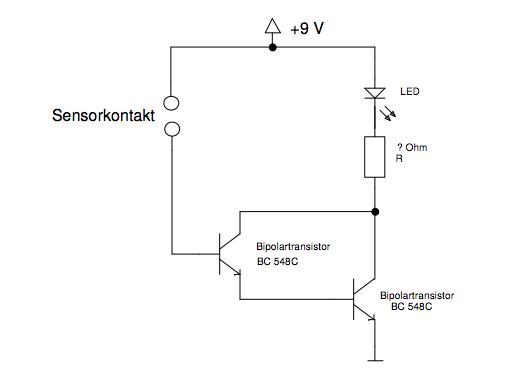
\includegraphics[width=\textwidth]{schaltbilder/darlington.png}
	\column{.48\textwidth}
	\begin{block}{Darlington-Schaltung}
		\begin{itemize}
		\item Der erste Transistor (Emitterfolger) verstärkt das Eingangssignal und gibt es auf die Basis des zweiten Transistors\\
		
		\item \emph{Vorteil:} größere Verstärkung, 
		auch sehr kleine Signale können verstärkt werden
		\end{itemize}
	\end{block}
	\end{columns}
\end{frame}
\begin{frame}
\begin{block}{Abschätzung der Verstärkung}
$I_{LED}\sim 15mA$\\
$R_{Finger}\simeq 5M\Omega \Rightarrow I_{Finger}=\frac{9V}{5M\Omega}=0.0018 mA$\\
$\Rightarrow \mathrm{Stromverst"arkung} \sim \frac{15mA}{0.0018mA}\sim 8500$
\end{block}
\end{frame}

\begin{frame}
\begin{block}{Astabile Kippstufe}
\centering
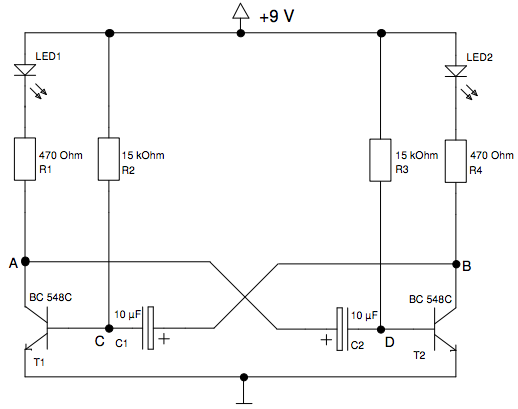
\includegraphics[width=.8\textwidth]{schaltbilder/blink.png}
\end{block}
\end{frame}
\begin{frame}
Beide Transistoren leiten abwechselnd $\Rightarrow$ eine Rechteckspannung an Punkten A und B
\end{frame}
\begin{frame}
	\begin{columns}
	\column{.48\textwidth}
	%\centering
	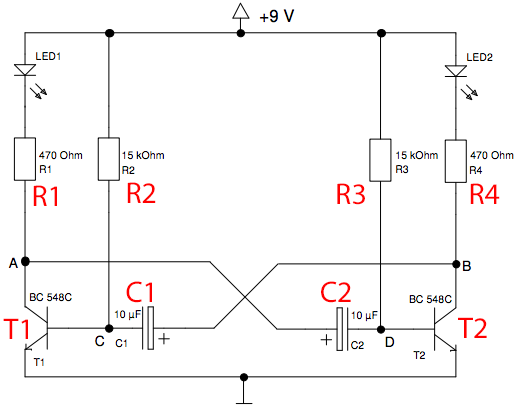
\includegraphics[width=\textwidth]{schaltbilder/blinkkommentar.png}
	\column{.48\textwidth}
	\begin{block}{Erster Zustand}
		\begin{itemize}
		\item Transistor $T1$ leitet $U_A \sim 0V$
		\item Kondensator C2 wird über T1 entladen
		\item Kondensator C1 läd auf bis an Basis von T2 $\sim0.7$V
		\end{itemize}
	\end{block}
	\begin{block}{Zweiter Zustand}
	\begin{itemize}
	\item Transistor $T2$ leitet $U_B \sim 0V$
	\item Kondensator C1 wird über T2 entladen 
	\item Kondensator C2 läd auf bis an Basis von T1 $\sim 0.7$V 
	\end{itemize}
	\end{block}
	\end{columns}
\end{frame}
\begin{frame}
Frequenz mit $15k\Omega$: $5.28Hz$
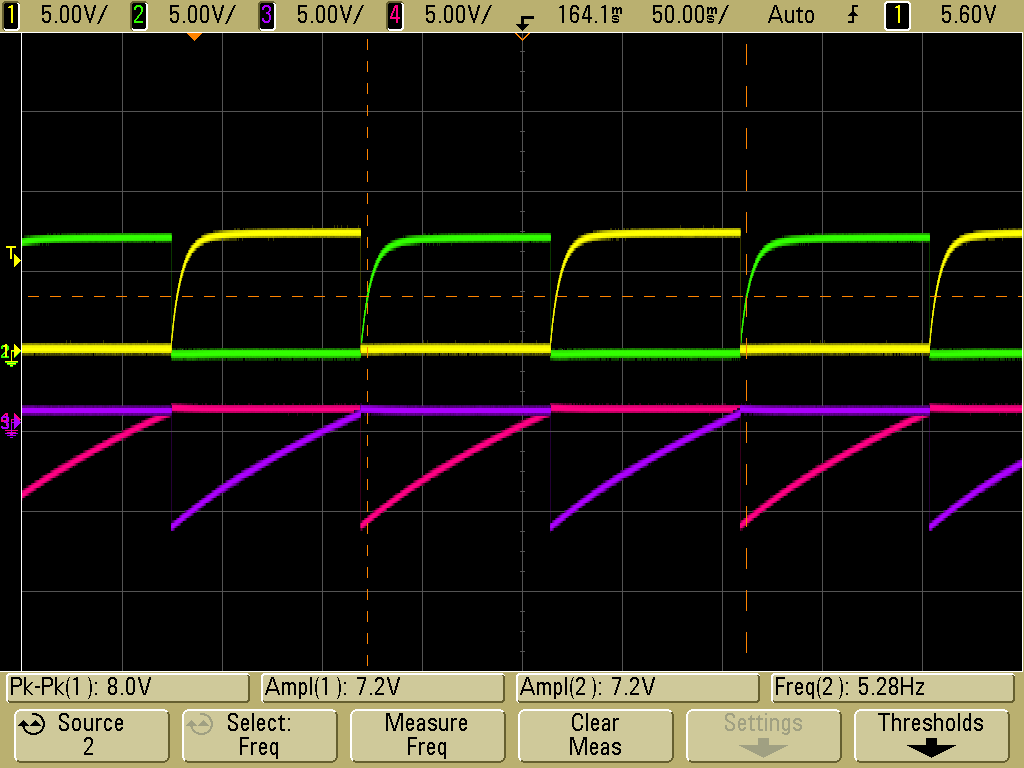
\includegraphics[width=.7\textwidth]{scope_43.png}
\end{frame}
\begin{frame}
Frequenz mit $220k\Omega$: $392mHz$
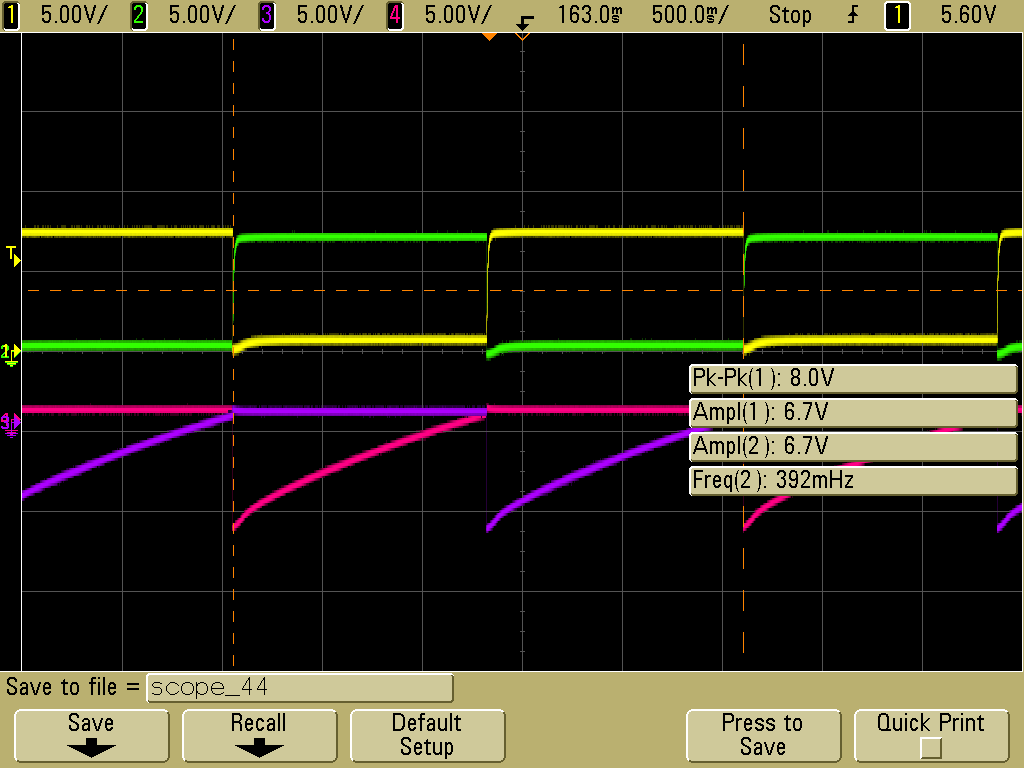
\includegraphics[width=.7\textwidth]{scope_44.png}
\end{frame}
\begin{frame}
\begin{block}{Impulsdauer}
\begin{itemize}
 \item mit $15k\Omega$ $t_1=0.7\cdot R2 \cdot C_2 = 0.7 \cdot 15k\Omega \cdot 10\mu F=0.105 s$ \\
 $\Rightarrow \sim 4.7 Hz$ gemessen $5.28Hz$
 \item mit $220k\Omega$ $t_1=0.7\cdot R2 \cdot C_2 = 0.7 \cdot 220k\Omega \cdot 10\mu F=1.54 s$\\
 $\Rightarrow \sim 0.32 Hz$ gemessen $0.39Hz$
\end{itemize}
\end{block}
\end{frame}
\end{document}
